\section{Collections, rules and protocol}\label{sec:data}

\subsection{Pair collections}\label{sec:collections}
Table~\ref{tab:collections} lists the eight collections (the seventh, the walks of all $19$ untouched recordings, contains the five recordings of the walk collection and fourteen more). A \emph{pair} is an ordered pair of variables with a known direction; the cause is the first variable of an edge of the documented graph. Two features of the table matter for every later statement. First, only T\"ubingen is a collection of unrelated mechanisms; the six others consist of pairs taken from one or two devices, so the number of \emph{distinct edges} is much smaller than the number of pair-runs (47 distinct edges behind the 94 i.i.d.\ chamber pair-runs, at most 65 distinct cause--effect names behind the 122 walk pairs, 8 behind the Bernoulli collection, 7 behind the changepoint collection and 4 behind the Malus collection, whose pairs share their cause variable). Intervals and tests that treat pairs as independent therefore overstate the information; Appendix Table~\ref{tab:collections_ci} gives cluster-bootstrap intervals (clusters: distinct edge, or recording for the walks). Second, in the chamber collections the cause is an actuator whose value the experimenter sets, which gives it a recognisable marginal law (uniform on a grid of levels, piecewise constant, a random walk) while the effects are sensors.

\begin{table}[t]
\caption{The eight real pair collections. ``Pairs'': pair-runs scored; ``edges'': distinct edges of the documented graph; ``units'': independent recordings or experiments. Rows: rows per pair after the cap of $2000$ random rows (T\"ubingen: at most $2000$ rows, dequantised; chamber collections: raw values).}
\label{tab:collections}
\small
\begin{tabular}{@{}lccccp{5.6cm}@{}}
\toprule
Collection & Pairs & Edges & Units & Rows & Source and cause\\
\midrule
T\"ubingen & 102 & 102 & 102 & $\le 2000$ & Univariate pairs of the CEP benchmark \citep{mooij2016distinguishing}; official weights\\
Chambers iid & 94 & 47 & 2 & 2000 & Wind and light tunnel with i.i.d.\ actuator settings \citep{gamella2025chamber}; two seeds per edge\\
Walks, all 19 & 486 & $\le65$ & 19 & 2000 & All untouched recordings (wind-tunnel random-walk actuators, the pressure-control recording, light-tunnel walks); every edge of each documented graph\\
Chambers walks & 122 & $\le65$ & 5 & 2000 & First recording of each type of random-walk experiments (actuators are random walks); the same cause--effect names recur across the five recordings\\
Sachs & 17 & 17 & 1 & 853 & Consensus arcs among 11 proteins, log scale \citep{sachs2005causal}\\
Bernoulli & 16 & 8 & 1 & 2000 & Wind tunnel, \texttt{random\_loads\_both}; the cause \texttt{load\_in} takes $101$ levels (steps of $0.01$), so after subsampling it has about $20$ rows per value; cause always \texttt{load\_in}\\
Changepoints & 70 & 7 & 10 & 2000 & Wind tunnel, piecewise-constant actuator (change points); cause always \texttt{load\_in}\\
Malus & 48 & 4 & 12 & 1000 & Light tunnel with polarisers, Malus's law; causes \texttt{pol\_1}, \texttt{pol\_2}\\
\bottomrule
\end{tabular}
\end{table}

Table~\ref{tab:diag} describes the collections with the quantities used later: the median number of rows, the median absolute Spearman correlation, the median residual heteroscedasticity $h$ of Section~\ref{sec:regimes} (true direction), the median excess kurtosis of the cause and of the effect, the median number of distinct values of the cause, and the share of pairs with many ties (fewer distinct values than $90\%$ of the rows) in either variable before any jitter (T\"ubingen is reported after dequantisation, hence zero). Figure~\ref{fig:examples} shows one randomly chosen pair per collection.

\begin{table}[t]
\caption{Descriptive diagnostics of the seven original collections (medians over pairs unless stated; the $486$-pair walk collection has the same kind of pairs as the walk collection).}
\label{tab:diag}
\small
\begin{tabular}{@{}lcccccccc@{}}
\toprule
Collection & Pairs & $n$ & $|\rho_S|$ & $h$ & kurt. cause & kurt. effect & distinct cause values & ties\\
\midrule
T\"ubingen & 102 & 392 & 0.50 & 0.18 & -0.2 & 0.2 & 392 & 0.00\\
Chambers iid & 94 & 2000 & 0.27 & 0.02 & -1.2 & -0.4 & 86 & 1.00\\
Chambers walks & 122 & 2000 & 0.26 & 0.08 & -1.2 & -0.6 & 255 & 1.00\\
Sachs & 17 & 853 & 0.08 & 0.08 & 3.1 & 2.3 & 276 & 1.00\\
Bernoulli & 16 & 2000 & 0.53 & 0.18 & -1.2 & -1.2 & 101 & 1.00\\
Changepoints & 70 & 1983 & 0.45 & 0.22 & -0.7 & -0.1 & 4 & 1.00\\
Malus & 48 & 1000 & 0.02 & 0.02 & -1.2 & -1.4 & 732 & 1.00\\
\bottomrule
\end{tabular}
\end{table}

\begin{figure}[t]
\centering
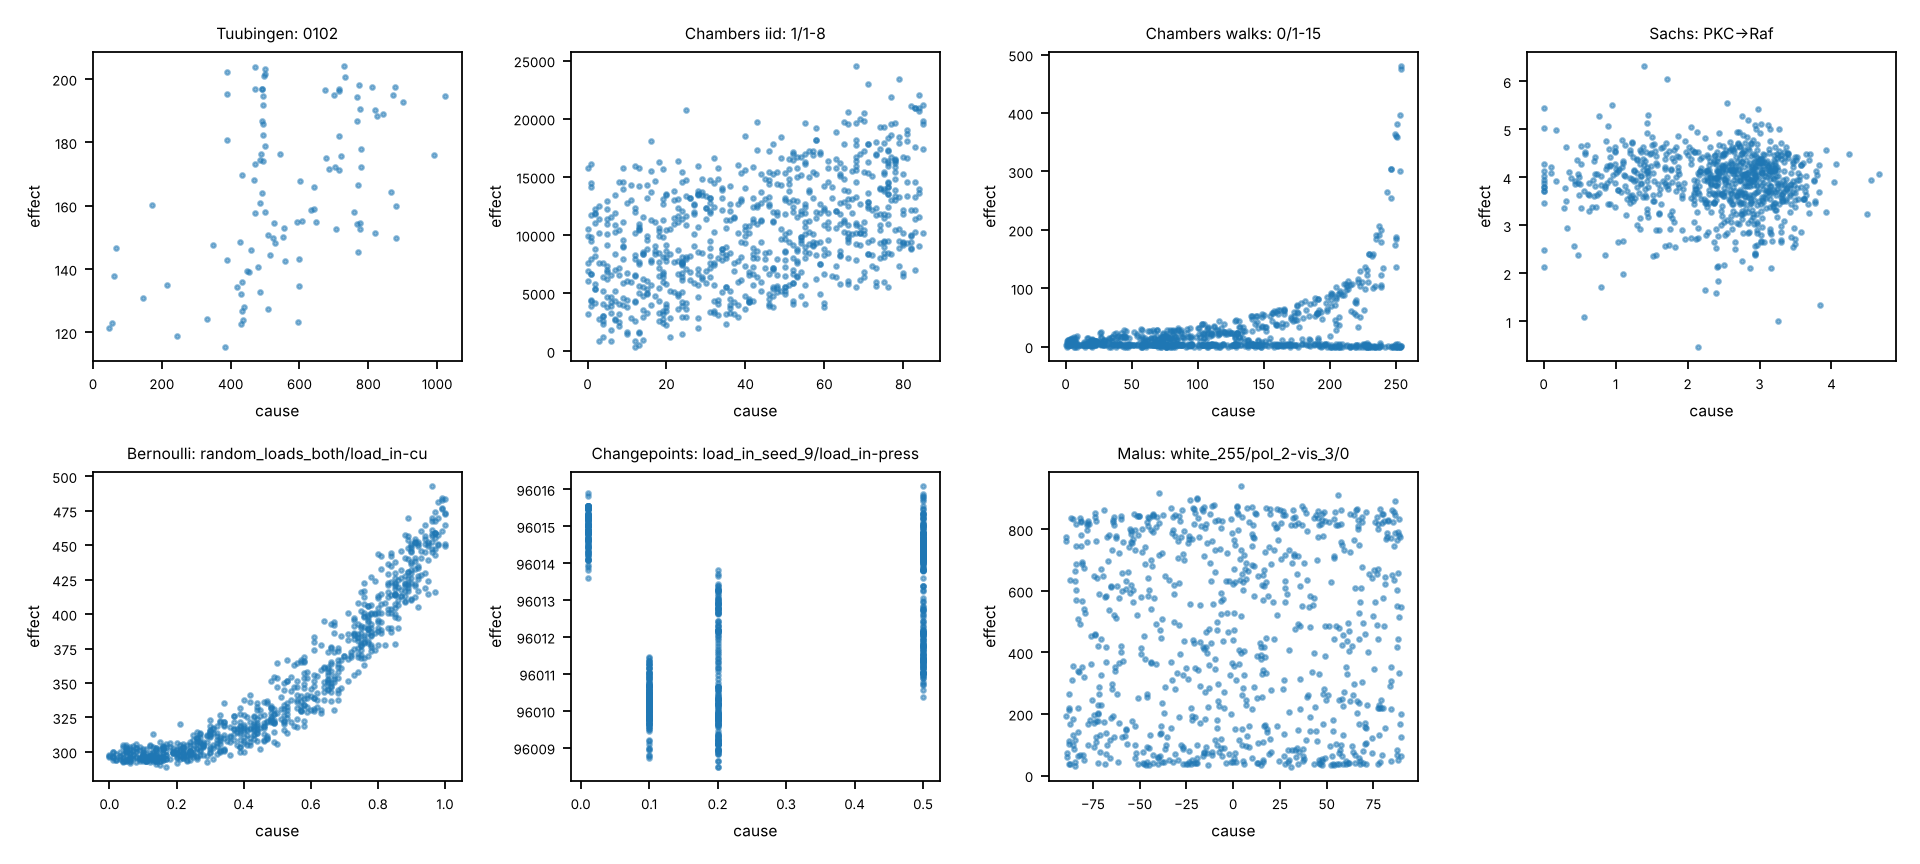
\includegraphics[width=\linewidth]{figs/examples.png}
\caption{One randomly chosen pair (seed $7$) from each collection; $800$ random rows, cause on the horizontal axis.}
\label{fig:examples}
\end{figure}

\subsection{Rules}\label{sec:rules}
Twelve rules, all run by us. Each returns a score whose sign gives the direction; a score of exactly zero counts as half correct. Settings were fixed in the script before the run (Appendix~\ref{app:prereg}) and none was tuned on a collection in which it is scored. \emph{Tie handling:} every rule receives the raw arrays (ties kept), as for the chambers in the first experiments; T\"ubingen arrays are dequantised (experiment 14) and have no ties. Giving the rules a copy with a $10^{-6}$ jitter on tied values reverses IGCI (Section~\ref{sec:ties}) and breaks TRA's spline fit, so jitter is used only in the sensitivity analysis of Section~\ref{sec:ties} and for the simulations.
\begin{itemize}
\item \textbf{IGCI} \citep{daniusis2010inferring}: entropy estimator with a uniform reference. \textbf{RECI} \citep{blobaum2018cause}: the direction with the smaller regression error of a spline fit after min--max scaling. Both are short re-implementations (\texttt{sprint\_cd/\allowbreak pair\_baselines.py}).
\item \textbf{ANM-HSIC} \citep{hoyer2009nonlinear}: additive-noise model with a spline regression and an HSIC independence test; \textbf{ANM-GP}: the \texttt{causal-learn} Gaussian-process version on $400$ rows; \textbf{RESIT} (\texttt{lingam}): random-forest regression of depth $4$ with $\alpha=0.01$.
\item \textbf{Pairwise LiNGAM} \citep{hyvarinen2013pairwise}: first-order likelihood-ratio statistic.
\item \textbf{LOCI} \citep{immer2023loci}: the authors' code in its default setting (neural networks, $5000$ steps, HSIC test, at most $1000$ rows).
\item \textbf{Compression} \citep{stienstra2026oneruler}: quantise both variables to $256$ levels, sort one by the other (stable), take the first difference as \texttt{int8}, compress with bzip2 (level 9), and compare the two normalised lengths. Two variants: our first implementation (\texttt{floor}$(256q)$, rows capped at $2000$) and the \emph{faithful} variant that reproduces the published figure (\texttt{round}$(255q)$, all rows thinned linearly above $8000$, raw values; Section~\ref{sec:audit}).
\item \textbf{TRA} \citep{elbouchattaoui2026tra}: cross-fitted smoothing-spline residuals, a rank-uniform residual cloud and the zero-dimensional persistence of its minimum spanning tree in a window; the constants $\kappa=1$, $c_\beta=4$, five folds, at most $1000$ rows are ours because the preprint does not fix them. It returns no value when the spline fit is ill-posed (cause with many tied values), which excludes it from the collections with binary or piecewise-constant causes.
\item \textbf{AVICI} \citep{lorch2022amortized}: the pretrained \texttt{scm-v0} model on the two-variable input, score $P(x\to y)-P(y\to x)$ (run in a separate environment with pinned JAX).
\item \textbf{PDM}: a gradient-boosting classifier trained on simulated pairs with $32$ features (ours; Appendix~\ref{app:negative}).
\end{itemize}
Reference implementations of IGCI, RECI, CDS, ANM and BivariateFit from the \texttt{cdt} package (v0.6.0, defaults) were also run to check ours (experiment 55; Section~\ref{sec:ties}). Not run: PNL (880\,s per pair on $400$ rows), CAM and SCORE (no package available offline), SLOPE (code not run), and rules that need the authors' trained weights.

\subsection{Protocol and provenance}\label{sec:protocol}
Every evaluation script was committed before it was run; Appendix~\ref{app:prereg} lists the 46 experiment scripts (numbers 17 to 60; 31 and 34 have two parts) with the commit that fixed them. Stored per-pair decisions are in \texttt{results/}, and every number in this paper is computed from them by the scripts in \texttt{scripts/}. Three analyses were designed after seeing per-pair results and are labelled as such where they appear: the multiverse and subset analyses of Sections~\ref{sec:multi}--\ref{sec:subsets}, the terciles of Table~\ref{tab:strata}, and the revised protocol of Section~\ref{sec:predict}. The study includes departures that we report rather than hide: our first compression implementation was wrong in a detail that the published text does not fix; the first run of the marginal-only classifier leaked information between training and test variables; one pre-registered test (Section~\ref{sec:predict}) was invalid as implemented and was rerun in a revised form, with both runs reported.
